\chapter{Technology Review}
\paragraph{In this section I'll examine the different technologies that were used in the application. I'll explain why I chose to implement each one specifically and whether or not I feet they were the right choice. As well as the major technologies used I'll touch on frameworks or libraries I feel are relevant to mention for the corresponding technology. The core technologies used that I will scrutinize the most in this section are; Spring Boot, React, MongoDB and Heroku.}

\section{MongoDB}
\paragraph{MongoDB is a NoSQL document oriented database program. A MongoDB database can contain multiple collections, each record in a collection is document. Documents are a structure composed of file and value pairs, similar to JSON objects or other mapping data types \cite{Mongo:doc}. The table below (Figure ~\ref{mongo2_label}) illustrates some differences between a MongoDB database and a relational database.}
\paragraph{Not only Sequential Query Language (NoSQL) is a database type that provides a mechanism for storage and retrieval of data which is modelled by means other than the tabular relations used in relational databases, in the case of MongoDB, it is document based. NoSQL databases are a favored solution for 'Big Data' storage as they incorporate a schema-less data model \cite{wiki:nosql}. 'Schema-less' means the database doesn't have fixed data structure. A NoSQL database provides increased scalability and flexibility compared to relational databases.}
\begin{figure}[h]
    \centering
    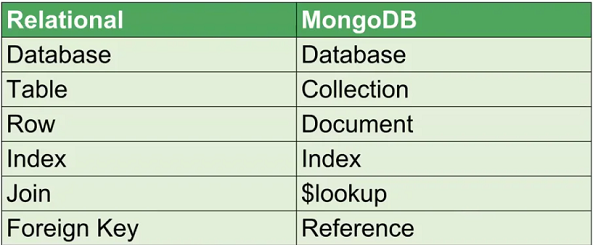
\includegraphics[scale=0.4]{Images/mongo2.png} 
    \label{mongo2_label}
    \caption{MongoDB vs relational DB}
\end{figure}

\subsection{MongoDB Atlas}
\paragraph{MongoDB Atlas is a cloud based system developed by MongoDB. Atlas provides an easy way to host and manage your data in the cloud with the service provider of your choice, for this application, I used Amazon Web Services (AWS).}
\paragraph{Atlas uses clusters to manage the data in a MongoDB project. Clusters are simply Atlas-managed MongoDB deployments and can be either a replica-set or a sharded cluster \cite{Mongo:clusters}. (Figure ~\ref{mongo3_label}) shows my atlas project is a replica set with three nodes}
\begin{figure}[h]
    \centering
    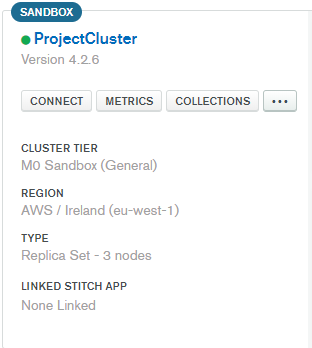
\includegraphics[scale=0.4]{Images/mongo3.png} 
    \label{mongo3_label}
    \caption{My MongoDB Project Cluster}
\end{figure}
\paragraph{A replica-set means there are multiple instances (in my case three) of MongoDB which each mirror all the data of the other. A replica-set consists of one primary node (master) and one or more secondary nodes (slaves). Read-operations can be served by any slave, but write-operations always take place on the master of the replica-set and are then propagated to the slaves. Replica-sets offer fault-tolerance as when one of the members of the replica-set goes down, the others take over. When the master goes down, the slaves will elect a new master.}
\newpage
\subsubsection{Atlas In My Application}
\paragraph{To connect my Spring Boot application to my MongoDB cluster I simply had to configure it's connection address in the 'application.properties' file (Figure ~\ref{mongo5_label}). }
\begin{figure}[ht]
    \centering
    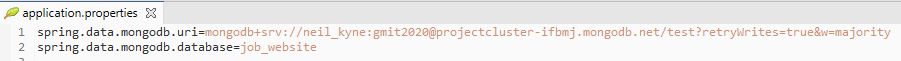
\includegraphics[scale=0.515]{Images/mongo5.png} 
    \label{mongo5_label}
    \caption{Connecting to My MongoDB Cluster}
\end{figure}
\paragraph{After providing the connection details above, our database, collection and all of the documents associated with that collection can be viewed on the MongoDB Atlas project page (Figure ~\ref{mongo1_label}).}
\begin{figure}[ht]
    \centering
    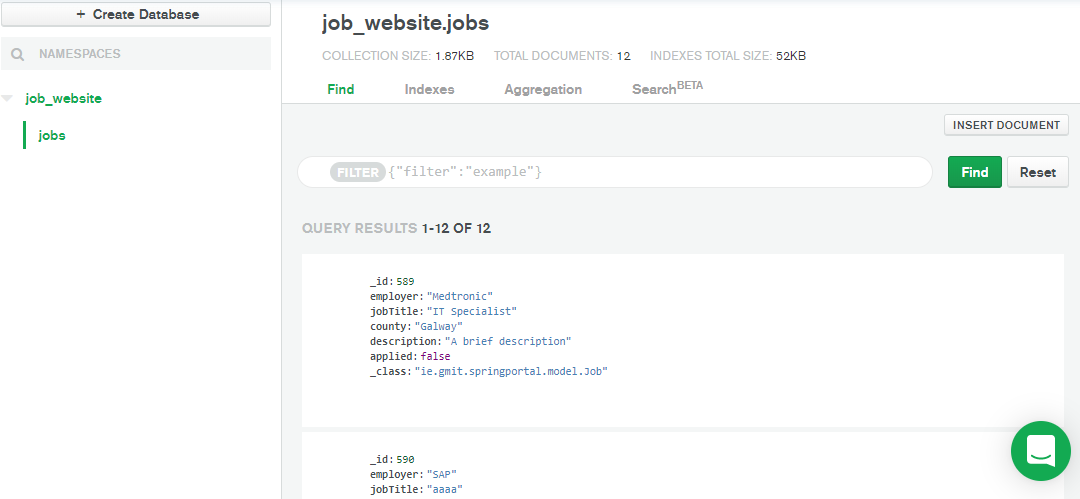
\includegraphics[scale=0.4]{Images/mongo1.png} 
    \label{mongo1_label}
    \caption{My MongoDB Database}
\end{figure}

\section{}
